\usepackage[a4paper,inner=27mm,outer=23mm,top=24mm,bottom=27mm,headheight=22pt]{geometry}
\usepackage[spanish,es-nodecimaldot]{babel}
\usepackage{fontspec}
\setmainfont{Libertinus Serif}
\setsansfont{Libertinus Sans}
\usepackage{microtype}
\usepackage{xcolor}
\usepackage{enumitem}
\usepackage{etoolbox}
\usepackage{tabularx}
\usepackage{longtable}
\usepackage{needspace}
\usepackage{fancyhdr}
\usepackage{graphicx}
\usepackage{caption}
\usepackage{accsupp}
\usepackage{hyperref}
\usepackage{hyperxmp}
\usepackage{bookmark}
\usepackage[most]{tcolorbox}
\usepackage{tikz}
\usetikzlibrary{arrows.meta,calc,decorations.pathreplacing,fit,positioning,shapes.geometric}

\definecolor{CourseNavy}{HTML}{24364B}
\definecolor{CourseBlue}{HTML}{446A8C}
\definecolor{CourseTeal}{HTML}{4F7F7B}
\definecolor{CourseAmber}{HTML}{A9713A}
\definecolor{CourseRed}{HTML}{965B59}
\definecolor{CourseInk}{HTML}{252A30}
\definecolor{CourseMuted}{HTML}{5D6670}
\definecolor{CourseRule}{HTML}{D8E0E7}
\definecolor{CoursePaper}{HTML}{FBFCFD}
\definecolor{CoursePaleBlue}{HTML}{F4F7FA}
\definecolor{CoursePaleTeal}{HTML}{F3F8F7}
\definecolor{CoursePaleAmber}{HTML}{FBF7F0}
\definecolor{CoursePaleRed}{HTML}{FAF4F3}
\definecolor{CourseCoverMist}{HTML}{EDF2F5}


\RequirePackage{amsmath}
\RequirePackage{amssymb}
\RequirePackage{amsthm}
\RequirePackage{mathtools}

\providecommand{\N}{\mathbb{N}}
\providecommand{\Z}{\mathbb{Z}}
\providecommand{\Q}{\mathbb{Q}}
\providecommand{\R}{\mathbb{R}}
\providecommand{\Nzero}{\mathbb{N}_0}
\providecommand{\Img}{\operatorname{Im}}
\providecommand{\Dom}{\operatorname{Dom}}
\providecommand{\Cod}{\operatorname{Cod}}
\providecommand{\id}{\operatorname{id}}

\providecommand{\CanonicalUnit}[3]{\ignorespaces}
\providecommand{\ProofRole}[2]{\ignorespaces}

\theoremstyle{definition}
\newtheorem{definicion}{Definición}[chapter]
\newtheorem{ejemplo}[definicion]{Ejemplo}

\theoremstyle{plain}
\newtheorem{teorema}[definicion]{Teorema}
\newtheorem{proposicion}[definicion]{Proposición}
\newtheorem{corolario}[definicion]{Corolario}

\theoremstyle{remark}
\newtheorem{observacion}[definicion]{Observación}
\newtheorem{advertencia}[definicion]{Advertencia}

\renewcommand{\proofname}{Demostración}

\newcommand{\NumberSystemsVisual}{%
\begin{center}
\begin{tikzpicture}[font=\small, every node/.style={align=center}]
  \draw[CourseNavy,very thick,rounded corners=8pt,fill=CoursePaleBlue]
    (-4.7,-2.1) rectangle (4.7,2.1);
  \node[anchor=north west,text=CourseNavy,font=\bfseries] at (-4.45,1.9) {$\R$};
  \draw[CourseTeal,very thick,rounded corners=8pt,fill=CoursePaleTeal]
    (-3.5,-1.45) rectangle (2.1,1.45);
  \node[anchor=north west,text=CourseTeal,font=\bfseries] at (-3.25,1.25) {$\Q$};
  \draw[CourseBlue,very thick,rounded corners=8pt,fill=white]
    (-2.55,-0.9) rectangle (1.1,0.9);
  \node[anchor=north west,text=CourseBlue,font=\bfseries] at (-2.3,0.72) {$\Z$};
  \draw[CourseAmber,very thick,rounded corners=8pt,fill=CoursePaleAmber]
    (-1.55,-0.42) rectangle (0.2,0.42);
  \node[text=CourseAmber,font=\bfseries] at (-0.68,0) {$\N$};
  \node[text=CourseNavy] at (3.15,0.25) {irracionales};
  \node[text=CourseNavy] at (3.15,-0.25) {$\sqrt{2},\,\pi,\ldots$};
\end{tikzpicture}

\small\itshape Lectura del diagrama: cada sistema interior está contenido en
el siguiente; la región de $\R$ situada fuera de $\Q$ representa los
irracionales.
\end{center}%
}

\newcommand{\DistanceNeighbourhoodVisual}{%
\begin{center}
\begin{tikzpicture}[x=1.3cm,y=1cm,font=\small]
  \draw[-{Latex[length=2mm]},CourseInk] (-3.2,0) -- (3.2,0);
  \draw[CourseBlue,line width=4pt] (-1.94,0) -- (1.94,0);
  \draw[CourseBlue,very thick,fill=white] (-2,0) circle (2.8pt);
  \draw[CourseBlue,very thick,fill=white] (2,0) circle (2.8pt);
  \draw[CourseInk] (0,-0.12)--(0,0.12);
  \node[below=5pt] at (-2,0) {$a-r$};
  \node[below=5pt] at (0,0) {$a$};
  \node[below=5pt] at (2,0) {$a+r$};
  \fill[CourseBlue] (0,0) circle (1.8pt);
  \draw[CourseAmber,thick,{Latex[length=2mm]}-{Latex[length=2mm]}]
    (0,0.58)--(1.35,0.58);
  \node[above,text=CourseAmber] at (0.68,0.58) {$|x-a|$};
  \fill[CourseAmber] (1.35,0) circle (1.8pt);
  \node[below=5pt,text=CourseAmber] at (1.35,0) {$x$};
  \node[above=3pt,text=CourseBlue] at (-1.35,0) {$V_r(a)$};
\end{tikzpicture}

\small\itshape Lectura del diagrama: $V_r(a)=(a-r,a+r)$ es abierto. Los
círculos huecos excluyen $a-r$ y $a+r$; $|x-a|<r$ sitúa a $x$ dentro del
entorno y la longitud destacada es la distancia entre $x$ y $a$.
\end{center}%
}

\newcommand{\FunctionMappingVisual}{%
\begin{center}
\begin{tikzpicture}[font=\small,>=Latex]
  \node[draw=CourseBlue,very thick,ellipse,minimum width=2.6cm,minimum height=4.3cm,
    fill=CoursePaleBlue,label=above:{\bfseries dominio $A$}] (A) at (-3,0) {};
  \node[draw=CourseTeal,very thick,ellipse,minimum width=3.1cm,minimum height=4.3cm,
    fill=CoursePaleTeal,label=above:{\bfseries codominio $B$}] (B) at (3,0) {};
  \coordinate (a1) at (-3,1.1); \coordinate (a2) at (-3,0); \coordinate (a3) at (-3,-1.1);
  \coordinate (b1) at (3,1.25); \coordinate (b2) at (3,0.35); \coordinate (b3) at (3,-0.55); \coordinate (b4) at (3,-1.35);
  \foreach \p in {a1,a2,a3,b1,b2,b3,b4} \fill[CourseInk] (\p) circle (2.1pt);
  \draw[CourseNavy,thick,->] (a1) to[bend left=8] (b1);
  \draw[CourseNavy,thick,->] (a2) -- (b2);
  \draw[CourseNavy,thick,->] (a3) to[bend right=8] (b3);
  \draw[CourseAmber,thick,rounded corners] (2.55,1.6) rectangle (3.45,-0.95);
  \node[right,text=CourseAmber] at (3.55,0.2) {imagen $f(A)$};
  \node[text=CourseRed] at (3,-1.35) {$\bullet$};
  \node[right,text=CourseRed] at (3.18,-1.35) {no alcanzado};
\end{tikzpicture}

\small\itshape Lectura del diagrama: todas las flechas parten del dominio;
la imagen reúne los valores alcanzados y puede ser menor que el codominio.
\end{center}%
}


\newcommand{\SequenceCorridorVisual}{%
\begin{tikzpicture}[x=0.62cm,y=1.15cm,>=Latex]
  \draw[->,CourseInk] (0,0) -- (11.2,0) node[right] {$n$};
  \draw[->,CourseInk] (0,-0.15) -- (0,3.2) node[above] {$a_n$};
  \draw[CourseTeal,thick] (0,1.65) -- (10.8,1.65) node[right] {$L$};
  \draw[CourseAmber,dashed] (0,2.25) -- (10.8,2.25) node[right] {$L+\varepsilon$};
  \draw[CourseAmber,dashed] (0,1.05) -- (10.8,1.05) node[right] {$L-\varepsilon$};
  \draw[CourseBlue,densely dotted] (4.5,0) -- (4.5,2.85) node[above] {$N$};
  \foreach \x/\y in {1/2.8,2/0.45,3/2.45,4/0.82,5/2.12,6/1.22,7/1.92,8/1.42,9/1.8,10/1.52}{
    \fill[CourseNavy] (\x,\y) circle (1.7pt);
  }
  \draw[decorate,decoration={brace,amplitude=4pt},CourseTeal]
    (4.65,1.05) -- (4.65,2.25) node[midway,right=5pt,align=left] {corredor\\de radio $\varepsilon$};
\end{tikzpicture}%
}

\newcommand{\EpsilonDeltaVisual}{%
\begin{tikzpicture}[x=1.25cm,y=1.05cm,>=Latex]
  \fill[CoursePaleTeal] (-2.45,-0.72) rectangle (2.45,0.72);
  \fill[CoursePaleBlue] (-0.95,-1.85) rectangle (0.95,1.85);
  \draw[CourseAmber,dashed] (-2.55,0.72) -- (2.55,0.72) node[right] {$L+\varepsilon$};
  \draw[CourseAmber,dashed] (-2.55,-0.72) -- (2.55,-0.72) node[right] {$L-\varepsilon$};
  \draw[CourseBlue,densely dotted] (-0.95,-1.85) -- (-0.95,1.85) node[above] {$a-\delta$};
  \draw[CourseBlue,densely dotted] (0.95,-1.85) -- (0.95,1.85) node[above] {$a+\delta$};
  \draw[->,CourseInk] (-2.7,0) -- (2.75,0) node[right] {$x$};
  \draw[->,CourseInk] (0,-1.95) -- (0,2.05) node[above] {$y$};
  \draw[CourseNavy,thick,domain=-2.3:2.3,samples=80]
    plot (\x,{0.52*\x+0.12*\x*\x});
  \fill[CourseNavy] (0,0) circle (1.7pt) node[below right] {$(a,L)$};
  \node[CourseInk,align=center] at (1.65,-1.45) {$0<|x-a|<\delta$\\fuerza $|f(x)-L|<\varepsilon$};
\end{tikzpicture}%
}

\newcommand{\SecantTangentVisual}{%
\begin{tikzpicture}[x=1.58cm,y=1.38cm,>=Latex]
  \pgfmathsetmacro{\basea}{-0.8}
  \pgfmathsetmacro{\steph}{2.2}
  \pgfmathsetmacro{\pointb}{\basea+\steph}
  \pgfmathsetmacro{\fa}{0.25*\basea*\basea+1.0}
  \pgfmathsetmacro{\fb}{0.25*\pointb*\pointb+1.0}
  \pgfmathsetmacro{\mtan}{0.5*\basea}
  \pgfmathsetmacro{\msec}{(\fb-\fa)/\steph}
  \draw[->,CourseInk] (-2.35,0) -- (2.35,0) node[right] {$x$};
  \draw[->,CourseInk] (0,-0.55) -- (0,2.55) node[above] {$y$};
  \draw[CourseNavy,line width=1.1pt,domain=-2.2:2.25,samples=100]
    plot (\x,{0.25*\x*\x+1.0});
  \foreach \smallh/\shade in {1.35/55,0.72/32}{%
    \pgfmathsetmacro{\smallb}{\basea+\smallh}
    \pgfmathsetmacro{\smallfb}{0.25*\smallb*\smallb+1.0}
    \pgfmathsetmacro{\smallm}{(\smallfb-\fa)/\smallh}
    \draw[CourseAmber!\shade!CourseInk,densely dotted,line width=0.7pt,
      domain=-2.15:2.15] plot (\x,{\fa+\smallm*(\x-\basea)});
    \fill[CourseAmber!\shade!CourseInk] (\smallb,\smallfb) circle (1.35pt);
  }
  \draw[CourseAmber,dashed,line width=1.15pt,domain=-2.15:2.15]
    plot (\x,{\fa+\msec*(\x-\basea)});
  \draw[CourseTeal,line width=1.35pt,domain=-2.15:2.15]
    plot (\x,{\fa+\mtan*(\x-\basea)});
  \coordinate (A) at (\basea,\fa);
  \coordinate (B) at (\pointb,\fb);
  \fill[CourseNavy] (A) circle (2.2pt);
  \fill[CourseNavy] (B) circle (2.2pt);
  \draw[CourseRule] (\basea,0.05) -- (\basea,-0.05) node[below,CourseInk] {$a$};
  \draw[CourseRule] (\pointb,0.05) -- (\pointb,-0.05) node[below,CourseInk] {$a+h$};
  \node[CourseNavy,anchor=south east,fill=white,inner sep=1pt] at (A) {$(a,f(a))$};
  \node[CourseNavy,anchor=south west,fill=white,inner sep=1pt] at (B) {$(a+h,f(a+h))$};
  \node[CourseAmber,anchor=south west,fill=white,inner sep=1.5pt] at (-2.08,0.98) {secante};
  \node[CourseTeal,anchor=north west,fill=white,inner sep=1.5pt] at (1.10,0.36) {tangente};
  \draw[->,CourseBlue,line width=0.8pt] (\pointb,-0.34) -- (\basea,-0.34)
    node[midway,below,CourseInk] {$h\to0$};
  \node[CourseMuted,anchor=north west] at (-2.18,2.48) {$f(x)=\frac{x^2}{4}+1$};
\end{tikzpicture}%
}

\newcommand{\DerivativeSignVisual}{%
\begin{tikzpicture}[x=1.05cm,y=1cm,>=Latex]
  \draw[CourseInk,line width=0.7pt] (-3.2,1.45) -- (3.2,1.45);
  \foreach \x/\lab in {-1.25/a,1.25/b}{%
    \draw[CourseInk] (\x,1.55) -- (\x,1.35) node[below=4pt] {$\lab$};
  }
  \node[CourseTeal,font=\bfseries] at (-2.2,1.90) {$f'>0$};
  \node[CourseRed,font=\bfseries] at (0,1.90) {$f'<0$};
  \node[CourseTeal,font=\bfseries] at (2.2,1.90) {$f'>0$};
  \node[CourseMuted,anchor=east] at (-3.3,1.45) {signo};
  \node[CourseMuted,anchor=east] at (-3.3,0.15) {variación};
  \draw[CourseTeal,very thick,->] (-3.0,-0.25) -- (-1.35,0.70);
  \draw[CourseRed,very thick,->] (-1.15,0.70) -- (1.15,-0.35);
  \draw[CourseTeal,very thick,->] (1.35,-0.35) -- (3.0,0.55);
  \fill[CourseNavy] (-1.25,0.76) circle (2.2pt);
  \fill[CourseNavy] (1.25,-0.41) circle (2.2pt);
  \node[CourseNavy,anchor=east] at (-1.58,0.76) {máximo local};
  \node[CourseNavy,anchor=west] at (1.58,-0.41) {mínimo local};
  \node[CourseInk,anchor=north,align=center,text width=11.7cm] at (0,-1.18)
    {El signo en cada intervalo determina la variación;\\
     los puntos candidatos deben clasificarse.};
\end{tikzpicture}%
}

\newcommand{\FunctionStudyWorkflowVisual}{%
\begin{tikzpicture}[x=1cm,y=1cm,>=Latex,
  workflowstep/.style={draw=CourseBlue,rounded corners=1.2mm,fill=CoursePaleBlue,
    minimum height=11mm,text width=34mm,align=center,font=\small,inner sep=4pt},
  check/.style={draw=CourseTeal,rounded corners=1.2mm,fill=CoursePaleTeal,
    minimum height=11mm,text width=34mm,align=center,font=\small,inner sep=4pt}]
  \node[workflowstep] (domain) at (-4.4,1.25) {Dominio y simetrías};
  \node[workflowstep] (limits) at (0,1.25) {Límites y asíntotas};
  \node[workflowstep] (first) at (4.4,1.25) {Signo de $f'$ y extremos};
  \node[workflowstep] (second) at (4.4,-0.55) {Signo de $f''$ e inflexión};
  \node[check] (graph) at (0,-0.55) {Predicción y representación};
  \node[check] (verify) at (-4.4,-0.55) {Comprobación de coherencia};
  \draw[->,CourseNavy,thick] (domain) -- (limits);
  \draw[->,CourseNavy,thick] (limits) -- (first);
  \draw[->,CourseNavy,thick] (first) -- (second);
  \draw[->,CourseNavy,thick] (second) -- (graph);
  \draw[->,CourseNavy,thick] (graph) -- (verify);
  \draw[->,CourseAmber,dashed,line width=0.9pt]
    (verify.south) -- ++(0,-0.75) -- ++(8.8,0) -- (first.south);
  \node[CourseAmber,fill=white,inner sep=2pt,font=\scriptsize]
    at (0,-2.03) {si aparece una incoherencia, revisar las decisiones anteriores};
\end{tikzpicture}%
}

\newcommand{\TaylorApproximationVisual}{%
\begin{center}
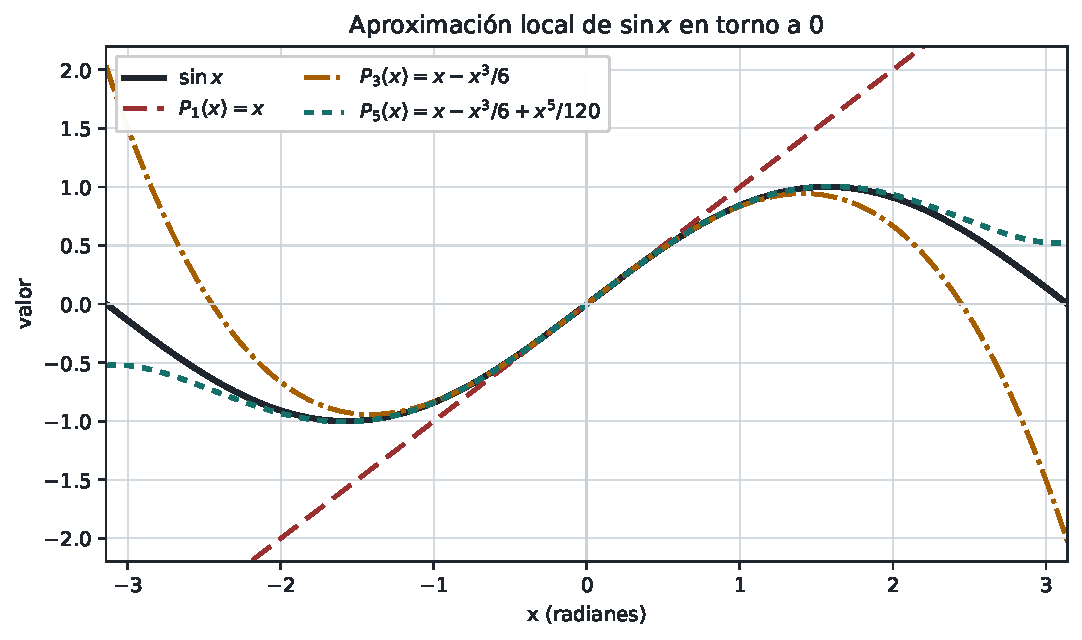
\includegraphics[width=0.94\linewidth]{src/theory/assets/plots/taylor_approximation.pdf}

\small\itshape Lectura del gráfico: cerca de cero, los polinomios de mayor
grado siguen al seno durante un intervalo más amplio. La comparación sigue
siendo local; no afirma una igualdad global.
\end{center}%
}

\newcommand{\TaylorErrorVisual}{%
\begin{center}
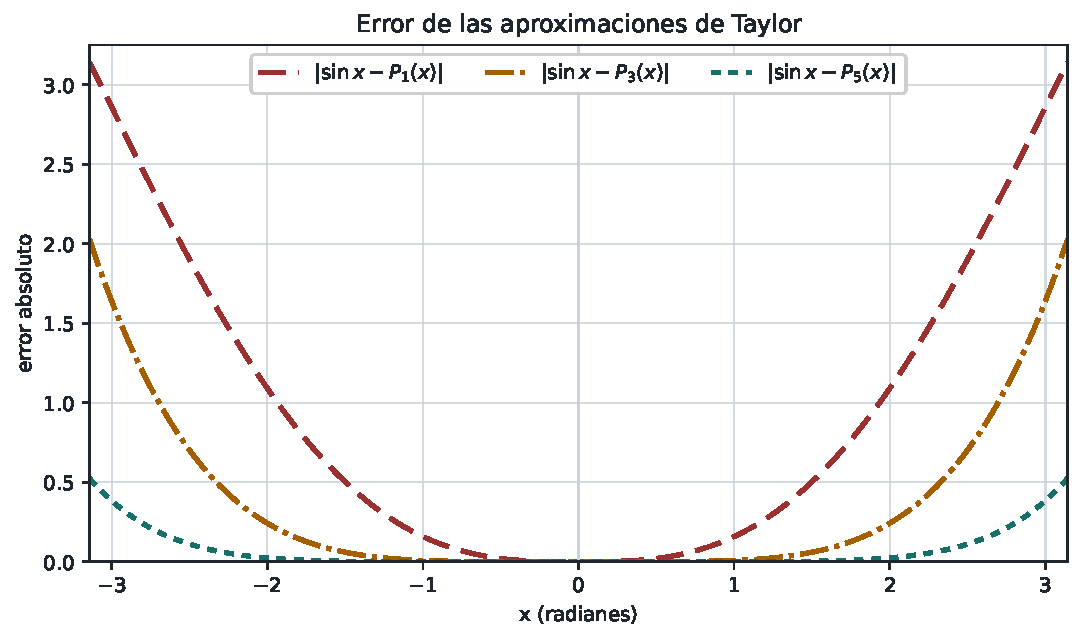
\includegraphics[width=0.94\linewidth]{src/theory/assets/plots/taylor_error.pdf}

\small\itshape Lectura del gráfico: el error se anula en el centro y crece al
alejarse. Comparar grados requiere fijar el mismo punto o intervalo; la forma
de las curvas hace visible esa condición.
\end{center}%
}


\hypersetup{
  colorlinks=true,
  hypertexnames=false,
  linkcolor=CourseBlue,
  urlcolor=CourseTeal,
  pdftitle={Cálculo Diferencial en una Variable — Teoría — Edición pública para estudiantes · v1.0},
  pdfauthor={Giovanni Dalmasso, PhD},
  pdfsubject={Libro de teoría para un primer curso de cálculo diferencial · Handle DAU: https://hdl.handle.net/20.500.14342/7180},
  pdfkeywords={cálculo diferencial, matemáticas aplicadas, teoría},
  pdfcreator={LuaLaTeX; fuente pública para estudiantes},
  pdfcopyright={Copyright © 2026 Giovanni Dalmasso},
  pdflicenseurl={https://creativecommons.org/licenses/by-sa/4.0/},
  pdfmetalang={es},
  pdflang={es-ES},
  pdfdisplaydoctitle=true,
  keeppdfinfo=true,
  bookmarksopen=true,
  bookmarksnumbered=true
}
\pdfstringdefDisableCommands{\def\({}\def\){}\def\texttt#1{#1}}

\setlist[itemize]{leftmargin=*,itemsep=2pt,topsep=4pt}
\setlist[enumerate]{leftmargin=*,itemsep=2pt,topsep=4pt}
\setlength{\parindent}{0pt}
\setlength{\parskip}{4.2pt plus 1pt minus 1pt}
\raggedbottom
\emergencystretch=2em
\pretocmd{\section}{\Needspace{0.30\textheight}}{}{}
\pretocmd{\subsection}{\Needspace{0.24\textheight}}{}{}

\pagestyle{fancy}
\fancyhf{}
\fancyhead[L]{\small\sffamily Edición pública para estudiantes · v1.0}
\fancyhead[R]{\small\sffamily Cálculo Diferencial en una Variable}
\fancyfoot[C]{\thepage}
\renewcommand{\headrulewidth}{0.35pt}
\renewcommand{\headrule}{\hbox to\headwidth{\color{CourseRule}\leaders\hrule height \headrulewidth\hfill}}
\renewcommand{\chaptername}{Capítulo}

\newtcolorbox{EditionUnitCard}[1]{
  enhanced,breakable,frame hidden,boxrule=0pt,colback=white,
  borderline west={2.1pt}{0pt}{CourseTeal},
  title={#1},title after break={#1 (continuación)},fonttitle=\sffamily\bfseries,
  coltitle=CourseInk,left=8pt,right=2pt,top=4pt,bottom=3pt,
  before skip=8pt,after skip=7pt
}
\newtcolorbox{EditionNotice}[2][]{
  enhanced,breakable,frame hidden,boxrule=0pt,
  borderline west={1.8pt}{0pt}{CourseTeal},
  colback=CoursePaleTeal,coltitle=CourseInk,title={#2},fonttitle=\sffamily\bfseries,
  left=8pt,right=8pt,top=4pt,bottom=5pt,before skip=7pt,after skip=7pt,#1
}
\newtcolorbox{EditionWarningBox}[1]{
  enhanced,breakable,frame hidden,boxrule=0pt,
  borderline west={1.8pt}{0pt}{CourseAmber},
  colback=CoursePaleAmber,coltitle=CourseInk,title={#1},fonttitle=\sffamily\bfseries,
  left=8pt,right=8pt,top=4pt,bottom=5pt,before skip=6pt,after skip=6pt
}
\newtcolorbox{EditionCheckpointBox}[1]{
  enhanced,breakable,frame hidden,boxrule=0pt,
  borderline west={1.8pt}{0pt}{CourseTeal},
  colback=CoursePaleTeal,coltitle=CourseInk,title={#1},fonttitle=\sffamily\bfseries,
  left=8pt,right=8pt,top=4pt,bottom=5pt,before skip=6pt,after skip=6pt
}

\newcommand{\StudySignal}[1]{%
  \par\smallskip\noindent
  \textcolor{CourseTeal}{\rule{2pt}{1.12em}}\hspace{6pt}%
  \textbf{Clave de estudio.} #1\par\smallskip
}

\tcolorboxenvironment{definicion}{
  enhanced,breakable,frame hidden,boxrule=0pt,colback=CoursePaleBlue,
  borderline west={1.8pt}{0pt}{CourseBlue},
  left=7pt,right=7pt,top=4pt,bottom=4pt,before skip=7pt,after skip=7pt
}
\tcolorboxenvironment{teorema}{
  enhanced,breakable,frame hidden,boxrule=0pt,colback=CoursePaleTeal,
  borderline west={1.8pt}{0pt}{CourseTeal},
  left=7pt,right=7pt,top=4pt,bottom=4pt,before skip=7pt,after skip=7pt
}
\tcolorboxenvironment{proposicion}{
  enhanced,breakable,frame hidden,boxrule=0pt,colback=CoursePaleTeal,
  borderline west={1.8pt}{0pt}{CourseTeal},
  left=7pt,right=7pt,top=4pt,bottom=4pt,before skip=7pt,after skip=7pt
}
\tcolorboxenvironment{advertencia}{
  enhanced,breakable,frame hidden,boxrule=0pt,colback=CoursePaleAmber,
  borderline west={1.8pt}{0pt}{CourseAmber},
  left=7pt,right=7pt,top=4pt,bottom=4pt,before skip=7pt,after skip=7pt
}
\tcolorboxenvironment{ejemplo}{
  enhanced,breakable,colback=CoursePaper,colframe=CourseRule,
  boxrule=0.45pt,left=7pt,right=7pt,top=4pt,bottom=4pt,
  before skip=7pt,after skip=7pt
}

\newcommand{\RegisteredBookFigure}[5]{%
  \par\medskip
  \begin{minipage}{\linewidth}
  \centering
  \refstepcounter{figure}%
  \hypertarget{figure:#1}{}%
  \label{#2}%
  \BeginAccSupp{method=pdfstringdef,unicode,ActualText={#4}}%
  #5%
  \EndAccSupp{}%
  \captionsetup{type=figure}%
  \caption*{\figurename~\thefigure. #3}%
  \end{minipage}
  \par\medskip
}
\newcommand{\StableFigureRef}[2]{figura~\ref{#2}}

\newcommand{\DeclareEditionOverlay}[2]{%
  \expandafter\long\expandafter\def\csname PublicOverlay@#1\endcsname{#2}%
}
\newcommand{\DispatchEditionOverlay}[3]{%
  \ifcsname PublicOverlay@#1\endcsname
    \csname PublicOverlay@#1\endcsname
  \else
    \PackageError{public-theory}{Missing Student overlay for unit #1}{}%
  \fi
}
\newcommand{\CanonicalChapterInput}[2]{\input{#2}}
\renewcommand{\CanonicalUnit}[3]{%
  \par\medskip
  \hypertarget{unit:#1}{}%
  \DispatchEditionOverlay{#1}{#2}{#3}%
  \ignorespaces
}

\newcommand{\DeclareStudentProofGuidance}[2]{%
  \expandafter\long\expandafter\def\csname PublicStudentProof@#1\endcsname{#2}%
}
\DeclareStudentProofGuidance{proof-002}{Reconstruye la demostración por contradicción de la irracionalidad de $\sqrt2$ y localiza el choque con la fracción reducida.}
\DeclareStudentProofGuidance{proof-003}{Sigue una vez la derivación de la desigualdad triangular; después úsala como herramienta de estimación.}
\DeclareStudentProofGuidance{proof-005}{Comprende una derivación representativa de estas identidades y conserva siempre sus condiciones de validez.}
\DeclareStudentProofGuidance{proof-006}{Reconstruye la lectura epsilon--$N$: dado el margen, produce un umbral que controle todos los términos posteriores.}
\DeclareStudentProofGuidance{proof-007}{Reconstruye los pasos esenciales de unicidad y de las reglas de cálculo, indicando dónde entra cada hipótesis.}
\DeclareStudentProofGuidance{proof-008}{Explica cómo monotonía, acotación y completitud se encadenan para obtener convergencia.}
\DeclareStudentProofGuidance{proof-009}{Aprende el criterio de Cauchy y decide cuándo permite concluir convergencia en $\R$.}
\DeclareStudentProofGuidance{proof-011}{Reconstruye las dos direcciones del criterio secuencial y distingue probar un límite de refutarlo.}
\DeclareStudentProofGuidance{proof-012}{Reconstruye una prueba epsilon--delta representativa respetando el orden de los cuantificadores.}
\DeclareStudentProofGuidance{proof-013}{Reconstruye el encaje geométrico que lleva a $\sin x/x$ y justifica el paso al límite.}
\DeclareStudentProofGuidance{proof-014}{Sigue una vez cómo se obtiene la continuidad de las familias elementales; después aplícala sin perder el dominio.}
\DeclareStudentProofGuidance{proof-015}{Conoce el enunciado de Weierstrass, comprueba compacto y continuidad, y distingue existencia de localización.}
\DeclareStudentProofGuidance{proof-016}{Explica la estrategia de intervalos encajados que garantiza un cero, sin confundir existencia con unicidad.}
\DeclareStudentProofGuidance{proof-017}{Reconstruye cómo el teorema del valor intermedio se reduce al caso de un cero y conserva sus hipótesis.}
\DeclareStudentProofGuidance{proof-018}{Reconstruye una derivada desde el cociente incremental y justifica el paso al límite.}
\DeclareStudentProofGuidance{proof-019}{Reconstruye las reglas de producto y cociente, señalando el término añadido y la condición del denominador.}
\DeclareStudentProofGuidance{proof-020}{Reconstruye la regla de la cadena separando el caso en que el incremento interior se anula.}
\DeclareStudentProofGuidance{proof-021}{Explica la estrategia de la derivada de la inversa y por qué la hipótesis $f'(a)\ne0$ es decisiva.}
\DeclareStudentProofGuidance{proof-022}{Sigue una vez la derivación logarítmica con sus restricciones; después úsala como técnica.}
\DeclareStudentProofGuidance{proof-023}{Reconstruye la demostración de Rolle desde el teorema de los extremos y el resultado de Fermat.}
\DeclareStudentProofGuidance{proof-024}{Reconstruye el teorema del valor medio aplicando Rolle a una función auxiliar adecuada.}
\DeclareStudentProofGuidance{proof-025}{Conoce las formas y las hipótesis de l'Hôpital; aplícalo solo tras verificar ambas.}
\DeclareStudentProofGuidance{proof-026}{Sigue una vez la justificación de los criterios de extremos; después clasifica con signos e hipótesis.}
\DeclareStudentProofGuidance{proof-027}{Sigue una vez la conexión entre cuerdas, variación de $f'$ y signo de $f''$; conserva la regularidad necesaria.}
\DeclareStudentProofGuidance{proof-028}{Reconstruye cómo las derivadas en el centro determinan los coeficientes y la unicidad del polinomio.}
\DeclareStudentProofGuidance{proof-029}{Comprende la función auxiliar y el uso del valor medio que producen el resto de Lagrange.}
\DeclareStudentProofGuidance{proof-030}{Conoce la cota de Lagrange, controla la derivada en todo el tramo y aplícala al error.}
\DeclareStudentProofGuidance{proof-032}{Explica por qué suma, producto y composición conservan el orden asintótico bajo las condiciones indicadas.}

\newcommand{\StudentProofCue}[2]{%
  \ifcsname PublicStudentProofSeen@#1\endcsname
  \else
    \expandafter\gdef\csname PublicStudentProofSeen@#1\endcsname{1}%
    \ifcsname PublicStudentProof@#1\endcsname
      \StudySignal{\csname PublicStudentProof@#1\endcsname}%
    \fi
  \fi
}
\renewcommand{\ProofRole}[2]{\StudentProofCue{#1}{#2}\ignorespaces}

\newtcolorbox{PublicXrefBox}[1]{
  enhanced,breakable,frame hidden,boxrule=0pt,
  borderline west={1.6pt}{0pt}{CourseTeal},
  colback=CoursePaleTeal,coltitle=CourseInk,title={#1},
  fonttitle=\small\sffamily\bfseries,fontupper=\small,
  left=7pt,right=7pt,top=3pt,bottom=4pt,before skip=7pt,after skip=8pt
}
\newcommand{\DeclarePublicXref}[2]{\expandafter\def\csname PublicXref@#1\endcsname{#2}}
\newcommand{\PublicXrefPendingUnit}{}
\newcommand{\PublicXrefRender}[1]{\ifcsname PublicXref@#1\endcsname\csname PublicXref@#1\endcsname\fi}
\newcommand{\PublicXrefFlushPending}{%
  \ifstrempty{\PublicXrefPendingUnit}{}{%
    \expandafter\PublicXrefRender\expandafter{\PublicXrefPendingUnit}%
    \global\let\PublicXrefPendingUnit\empty
  }%
}
